\chapter{Benchmark de Almacenamiento}\label{benchmark-de-almacenamiento}

La Tabla~\ref{tab:metricas-tdb} resume las métricas globales del array TileDB sparse con la configuración inicial (ZSTD-1) sobre datos1, previa al \textit{benchmark} de configuraciones de compresión.

\begin{table}[ht]
\centering
\begin{tabularx}{\textwidth}{>{\raggedright\arraybackslash}p{9.5cm}L}
\toprule
\textbf{Métrica} & \textbf{Valor} \\
\midrule
Pasos temporales & 20 \\
Resolución ráster & 34 200 $\times$ 23 040 px \\
Variables & H, QX, QY, MH \\
Celdas totales del dominio & 15 759 360 000 \\
Celdas almacenadas en TileDB & 1 311 695 098 \\
\% del dominio con agua & 8,3 \% \\
\addlinespace[6pt]
Ficheros GeoTIFF originales & 235 GB \\
TileDB sparse (ZSTD-1) & 19 GB \\
Espacio ahorrado & 216 GB (91,9 \%) \\
Ratio de compresión & 12,4$\times$ \\
\addlinespace[6pt]
Bytes/celda sin comprimir (4 vars $\times$ float32) & 16 B \\
Bytes/celda en TileDB & 15,6 B \\
Tiempo de carga (20 pasos) & 454 s ($\sim$7,5 min) \\
\bottomrule
\end{tabularx}
\caption{Métricas globales del array TileDB sparse con configuración inicial ZSTD-1 (datos1). La configuración definitiva tras el benchmark se recoge en la Tabla~\ref{tab:configuracion-final}.}
\label{tab:metricas-tdb}
\end{table}


El ahorro de espacio proviene principalmente del almacenamiento disperso (solo el $\sim$8,3 \% del dominio está inundado), no de la compresión en sí. Para cuantificar el impacto de distintas configuraciones de compresión se diseñó un \textit{benchmark} exhaustivo con cinco dimensiones de experimento, ejecutado sobre los datos reales del paso temporal 16\_00 (64,3 millones de celdas húmedas). Las lecturas se midieron sobre una región fija de 5 000$\times$5 000 celdas con 200 repeticiones para obtener resultados estadísticamente robustos.

\section{Entorno y metodología experimental}\label{entorno-y-metodologia-experimental}

Todos los experimentos se realizaron en la misma máquina para garantizar la comparabilidad de los resultados.

\subsection{Hardware y software}\label{hardware-y-software}

Hardware: procesador AMD Ryzen 9 7900X (12 núcleos / 24 hilos, 4,7--5,6 GHz), 32 GB de RAM DDR5 a 5200 MT/s, almacenamiento SSD (\textit{Solid-State Drive}) NVMe PCIe Gen4 de 2 TB.

Software: Windows 11 Pro con subsistema WSL2 (Ubuntu 24.04 LTS, kernel 6.6), Python 3.12.3, TileDB 0.36.1, NumPy 2.4.4, rasterio 1.5.0, Streamlit 1.36.

\subsection{Protocolo de medición}\label{protocolo-de-medicion}

Cada caso de prueba se ejecuta siguiendo el mismo protocolo:

\begin{itemize}
\item \textbf{Repeticiones.} Los \textit{benchmarks} de patrones de acceso (5 patrones en \texttt{benchmark\_queries.py} y 6 casos en \texttt{benchmark\_vs\_geotiff.py}) se ejecutan tres veces consecutivas y se reporta la mediana. Para el benchmark de filtros de compresión, en el que la dispersión es relevante para discriminar configuraciones similares, se ejecutaron 200 repeticiones sobre una región fija de 5 000$\times$5 000 celdas y se reporta mediana y desviación típica.

\item \textbf{Caché fría frente a caché caliente.} Antes de cada serie de repeticiones la caché de páginas del sistema operativo se libera con \texttt{sync \&\& echo 3 > /proc/sys/vm/drop\_caches} para medir el tiempo en frío de la primera lectura. Las repeticiones segunda y tercera se ejecutan sin liberar caché y miden el tiempo en caché caliente, que es el valor reportado en las tablas comparativas. La diferencia entre ambos tiempos cuantifica la sensibilidad de cada motor (TileDB y GeoTIFF) al estado de la caché del sistema operativo.

\item \textbf{Medición de RAM.} El consumo de memoria se mide con la biblioteca estándar \texttt{tracemalloc} de Python, registrando el pico de asignación entre el inicio y el fin de cada operación. Esta herramienta captura las asignaciones realizadas a través del asignador de Python, lo que incluye los arrays de NumPy devueltos por TileDB y rasterio. Los buffers internos asignados directamente en C (por ejemplo, los tiles descomprimidos por TileDB o las bandas leídas por GDAL antes de pasar a NumPy) no son visibles para \texttt{tracemalloc}, por lo que los valores reportados deben interpretarse como una cota inferior del consumo total del proceso, no como su valor exacto.

\item \textbf{Throughput.} Se calcula como $\text{bytes\_descomprimidos} / \text{tiempo\_caliente}$, donde \texttt{bytes\_descomprimidos} es el tamaño en memoria de los datos devueltos al cliente: $N_{\text{celdas}} \times N_{\text{variables}} \times 4$ bytes para float32. En TileDB sparse $N_{\text{celdas}}$ corresponde al número de celdas húmedas en la región consultada; en GeoTIFF es el tamaño completo de la ventana leída, incluyendo celdas secas.

\item \textbf{Reproducibilidad.} Todos los scripts de \textit{benchmark} están versionados en el directorio \texttt{spillway/} del proyecto y son reejecutables con un único argumento (\texttt{--dataset}). Los tiempos absolutos dependen del hardware; los factores relativos entre TileDB y GeoTIFF son los resultados directamente comparables.
\end{itemize}

\section{Resultado final: configuración definitiva}\label{resultado-final-configuracion-definitiva}

A partir de los resultados del \textit{benchmark} se generaron los 56 arrays definitivos (triton\_results/datos1--datos56) con el filtro ByteShuffle + ZSTD-9, manteniendo el resto de parámetros de producción (float32, tile 256$\times$256, array 3D con 1 fragmento por paso, multi-atributo).

El \textit{benchmark} evalúa cinco grupos de parámetros de forma independiente (G1--G5). La Tabla~\ref{tab:benchmark-resumen} resume las comparativas realizadas y la decisión adoptada en cada caso. Los resultados detallados se recogen en el Anexo B.

\begin{center}
\begin{tabularx}{\textwidth}{>{\raggedright\arraybackslash}p{3cm}>{\raggedright\arraybackslash}p{3.8cm}L>{\raggedright\arraybackslash}p{2.8cm}}
\toprule
\textbf{Grupo} & \textbf{Comparación} & \textbf{Resultado} & \textbf{Configuración elegida} \\
\midrule
G1.\\ Filtros & ZSTD puro (niveles 1, 3, 5, 9), ByteShuffle+ZSTD, BitShuffle+ZSTD & \textbullet~ByteShuffle+ZSTD-9: menor tamaño ($-$8,9 \% vs ZSTD-1). \newline \textbullet~Lectura similar entre variantes shuffle. & ByteShuffle+ZSTD-9 \\
G2.\\ Tile espacial & Tiles 256$\times$256, 512$\times$512 y 1\,024$\times$1\,024 celdas & \textbullet~Diferencias despreciables en tamaño y velocidad con datos dispersos. & 256$\times$256 \\
G3.\\ Tipo de dato & float64 (nativo GeoTIFF), float32, float16 & \textbullet~float16 no soportado. \newline \textbullet~float64: +9,4 \% sobre float32. \newline \textbullet~float32: equilibrio tamaño/precisión. & float32 \\
G4.\\ Estructura temporal & tile\_t=1 vs tile\_t=4; array 2D vs 3D & \textbullet~tile\_t=1: $-$19 \% frente a tile\_t=4. \newline \textbullet~1 fragmento/paso facilita el filtrado temporal. & Array 3D, 1 frag./paso \\
G5.\\ Atributos & 1 array multi-atributo vs 4 arrays independientes & \textbullet~Arrays separados: +14,9 \% en disco y 2,2$\times$ más lentos en lectura conjunta. & 1 array, 4 atributos \\
\bottomrule
\end{tabularx}
\captionsetup{hypcap=false}\captionof{table}{Resumen del benchmark de almacenamiento por grupos de parámetros.}
\label{tab:benchmark-resumen}
\end{center}


\begin{table}[ht]
\centering
\begin{tabularx}{\textwidth}{>{\raggedright\arraybackslash}p{5.5cm}LL}
\toprule
& \textbf{Configuración inicial (ZSTD-1)} & \textbf{Configuración final (ByteShuffle + ZSTD-9)} \\
\midrule
Tamaño total (20 pasos) & 19\,327 MB & 17\,613 MB \\
Ahorro respecto a configuración inicial & --- & \textbf{$-$1\,714 MB ($-$8,9\,\%)} \\
Mediana lectura región & $\sim$0,158 s & $\sim$0,196 s (similar) \\
Tiempo de carga & $\sim$454 s & $\sim$477 s \\
\bottomrule
\end{tabularx}
\caption{Comparativa entre la configuración inicial y la configuración final del array TileDB.}
\label{tab:configuracion-final}
\end{table}


La configuración final ocupa 1 714 MB menos (-8,9 \%) con tiempos de lectura equivalentes. El incremento de tiempo de carga (+22 s sobre 477 s totales) es asumible dado que la ingesta es un proceso puntual frente a la consulta continua de los datos.

Las herramientas de análisis y visualización construidas sobre el sistema se presentan en la sección~\ref{herramientas-desarrolladas}.

\section{Evaluación de rendimiento de las consultas analíticas}\label{evaluacion-rendimiento-consultas}

Para cuantificar el coste real de las consultas sobre el sistema definitivo, se midió el tiempo de ejecución de las principales funciones del motor analítico sobre \texttt{datos29}, el \textit{dataset} más voluminoso disponible (21 GB, 20 fragmentos, dominio de 34\,200\,$\times$\,23\,040 px). Las mediciones se realizaron en la máquina de desarrollo descrita en la Sección~\ref{hardware-y-software} (AMD Ryzen 9 7900X, 32 GB DDR5, SSD NVMe PCIe Gen4). Cada consulta se ejecutó una sola vez sobre caché fría, que es la condición real de uso: el usuario lanza una consulta bajo demanda sin garantía de que los datos estén en caché.

Las consultas se agrupan en tres categorías según su patrón de acceso a TileDB:

\begin{itemize}
\item \textbf{Instantáneas.} Acceden a un único fragmento (un paso temporal). Su coste es proporcional al número de celdas húmedas en ese instante.
\item \textbf{Multi-paso.} Recorren los 20 fragmentos secuencialmente acumulando un escalar o vector por paso. Son el grupo de mayor volumen de E/S.
\item \textbf{Acumuladas por píxel.} También recorren los 20 fragmentos, pero actualizan en cada paso un \textit{grid} de tamaño fijo $n_r \times n_c$ (sección~\ref{motor-de-consultas-analiticas}). Son las más costosas porque combinan E/S intensiva con escrituras dispersas en memoria.
\end{itemize}

La Figura~\ref{fig:patrones-acceso} ilustra estos tres patrones sobre el array TileDB. La Tabla~\ref{tab:benchmark-consultas} recoge los tiempos para el dominio completo y para un subdominio central del 50\,\% en cada eje (25\,\% del área total), que ilustra la ganancia cuando el usuario restringe la consulta a un área de interés mediante un \textit{bounding box}.

\begin{figure}[ht]
\centering
\begin{tikzpicture}[x=0.62cm, y=0.62cm, font=\small\sffamily]
  %% Tres paneles horizontales (tiempo × espacio), W=5 H=3 unidades
  %% Separación entre paneles: 1.5 unidades

  %% ---- Panel 1: Instantánea ----
  \fill[gray!10] (0,0) rectangle (5,3);
  \draw[gray!50, line width=0.8pt] (0,0) rectangle (5,3);
  % Banda vertical: un único paso temporal
  \fill[orange!45] (1.8,0) rectangle (2.35,3);
  \draw[orange!65!black, dashed, line width=0.7pt] (1.8,0) rectangle (2.35,3);
  % Ticks temporales
  \draw[gray!50, thin] (0,0) -- (0,-0.2) node[below, font=\tiny, gray!55] {$t_0$};
  \draw[gray!50, thin] (5,0) -- (5,-0.2) node[below, font=\tiny, gray!55] {$t_{19}$};
  \node[orange!65!black, font=\tiny\bfseries, below=0.15cm] at (2.1,0) {$t_k$};
  % Etiquetas
  \node[rotate=90, gray!50, font=\tiny] at (-0.55,1.5) {espacio};
  \node[orange!65!black, font=\small\bfseries, above=3pt] at (2.5,3) {Instantánea};
  \node[gray!60, font=\tiny, below=17pt] at (2.5,0) {Q1--Q6: 1 fragmento $\to$ $<$4 s};

  %% ---- Panel 2: Multi-paso (escalar) ----
  \def\px{6.5}
  \fill[gray!10] (\px,0) rectangle (\px+5,3);
  \draw[gray!50, line width=0.8pt] (\px,0) rectangle (\px+5,3);
  \fill[blue!22] (\px,0) rectangle (\px+5,3);
  \draw[gray!50, thin] (\px,0) -- (\px,-0.2) node[below, font=\tiny, gray!55] {$t_0$};
  \draw[gray!50, thin] (\px+5,0) -- (\px+5,-0.2) node[below, font=\tiny, gray!55] {$t_{19}$};
  \node[rotate=90, gray!50, font=\tiny] at (\px-0.55,1.5) {espacio};
  \node[blue!65!black, font=\small\bfseries, above=3pt] at (\px+2.5,3) {Escalar por paso};
  \node[gray!60, font=\tiny, below=17pt] at (\px+2.5,0) {Q11--Q14: 20 fragmentos $\to$ valor/paso};

  %% ---- Panel 3: Acumulada por píxel ----
  \def\qx{13}
  \fill[gray!10] (\qx,0) rectangle (\qx+5,3);
  \draw[gray!50, line width=0.8pt] (\qx,0) rectangle (\qx+5,3);
  \fill[red!18] (\qx,0) rectangle (\qx+5,3);
  % Flecha hacia mapa de resultado
  \draw[-Latex, red!65!black, line width=1pt] (\qx+5.2,1.5) -- (\qx+5.9,1.5);
  % Mini mapa 2D de salida (3×3, colores fijos)
  \fill[red!22]  (\qx+6.0,0.8)  rectangle +(0.32,0.32);
  \fill[red!35]  (\qx+6.35,0.8) rectangle +(0.32,0.32);
  \fill[red!48]  (\qx+6.7,0.8)  rectangle +(0.32,0.32);
  \fill[red!38]  (\qx+6.0,1.15) rectangle +(0.32,0.32);
  \fill[red!60]  (\qx+6.35,1.15)rectangle +(0.32,0.32);
  \fill[red!72]  (\qx+6.7,1.15) rectangle +(0.32,0.32);
  \fill[red!30]  (\qx+6.0,1.5)  rectangle +(0.32,0.32);
  \fill[red!55]  (\qx+6.35,1.5) rectangle +(0.32,0.32);
  \fill[red!80]  (\qx+6.7,1.5)  rectangle +(0.32,0.32);
  \draw[red!55!black, thin] (\qx+6.0,0.8) rectangle +(1.02,1.02);
  \node[red!55!black, font=\tiny, above=1pt] at (\qx+6.51,1.82) {mapa};
  \draw[gray!50, thin] (\qx,0) -- (\qx,-0.2) node[below, font=\tiny, gray!55] {$t_0$};
  \draw[gray!50, thin] (\qx+5,0) -- (\qx+5,-0.2) node[below, font=\tiny, gray!55] {$t_{19}$};
  \node[rotate=90, gray!50, font=\tiny] at (\qx-0.55,1.5) {espacio};
  \node[red!65!black, font=\small\bfseries, above=3pt] at (\qx+2.5,3) {Acumulada por píxel};
  \node[gray!60, font=\tiny, below=17pt] at (\qx+2.5,0) {Q7--Q9: 20 fragmentos $\to$ mapa 2D};
\end{tikzpicture}
\caption{Tres patrones de acceso al array TileDB según categoría de consulta. El eje horizontal representa el tiempo (20 fragmentos, uno por paso) y el eje vertical el espacio (dominio de simulación). La región coloreada indica los datos leídos. \textbf{Instantánea} (naranja): un único fragmento, proporcional al número de celdas húmedas en ese paso. \textbf{Escalar por paso} (azul): los 20 fragmentos, acumulando un valor numérico por paso. \textbf{Acumulada por píxel} (rojo): los 20 fragmentos actualizando un \textit{grid} $n_r \times n_c$ en cada paso, lo que genera los tiempos de 79--121 s observados en la Tabla~\ref{tab:benchmark-consultas}.}
\label{fig:patrones-acceso}
\end{figure}

\begin{table}[ht]
\centering
\begin{tabularx}{\textwidth}{>{\raggedright\arraybackslash}p{1.6cm}L>{\centering\arraybackslash}p{2.6cm}>{\centering\arraybackslash}p{2.6cm}}
\toprule
\textbf{Consulta} & \textbf{Descripción} & \textbf{Dom. completo (s)} & \textbf{Subdominio (s)} \\
\midrule
\multicolumn{4}{l}{\textit{Instantáneas (1 paso temporal, hora 60)}} \\[2pt]
Q2  & Serie temporal en un punto                & $<$\,0{,}1 & ---  \\
Q4  & Mapa de zonas inundadas                   & 2{,}9      & 0{,}6 \\
Q10a & Peligro para adultos                     & 3{,}8      & 1{,}0 \\
Q14 & Estadísticos por zona                     & ---        & 1{,}2 \\
Q15 & Semáforo de calado (3 niveles)            & 1{,}8      & 0{,}7 \\[4pt]
\multicolumn{4}{l}{\textit{Multi-paso (20 pasos temporales)}} \\[2pt]
Q5  & Evolución de la extensión inundada        & 31{,}5     & 13{,}9 \\
Q12 & Área inundada por hora                    & 31{,}2     & 13{,}8 \\[4pt]
\multicolumn{4}{l}{\textit{Acumuladas por píxel (20 pasos temporales)}} \\[2pt]
Q7  & Hora de llegada del frente de inundación  & 79{,}5     & 26{,}6 \\
Q8  & Duración total de la inundación           & 121{,}4    & 42{,}0 \\
Q9  & Hora de calado máximo                     & 98{,}3     & 33{,}7 \\
Q11 & Ventana para vehículos de emergencia      & 84{,}1     & 25{,}9 \\
\bottomrule
\end{tabularx}
\caption{Tiempos de ejecución de las consultas analíticas sobre \texttt{datos29} (21 GB). Subdominio: cuadrante central al 50\,\% en cada eje (25\,\% del área total). Caché fría, SSD NVMe PCIe Gen4, AMD Ryzen 9 7900X.}
\label{tab:benchmark-consultas}
\end{table}

Las consultas instantáneas responden en menos de 4 s incluso sobre el dominio completo. Las multi-paso tardan en torno a 30 s, determinadas principalmente por las 20 lecturas sucesivas a TileDB. Las acumuladas por píxel son las más lentas: oscilan entre 79,5 s (Q7) y 121,4 s (Q8) sobre el dominio completo. La restricción a un subdominio reduce los tiempos en un factor de 2--3$\times$, al decrecer proporcionalmente el número de celdas procesadas en cada fragmento.

\chapter{Herramientas Desarrolladas}\label{herramientas-desarrolladas}

Este capítulo describe las herramientas desarrolladas en torno al array TileDB: los scripts de consulta y visualización de escritorio, los \textit{benchmarks} de rendimiento y la aplicación web interactiva que expone el sistema al usuario final.

\section{Visualización rápida del dominio}\label{visualizador-interactivo}

El visualizador surge de una limitación práctica: renderizar un instante temporal completo cargando el array denso requeriría $\sim$3 GB por variable, superando la memoria disponible. La herramienta lee directamente del array TileDB sparse y proyecta las coordenadas de celdas húmedas al espacio de pantalla (máximo 4 096 px) sin materializar la cuadrícula completa. Encaja en el sistema como herramienta de exploración visual que no requiere exportación previa de datos.

Soporta cuatro modos: calado H (escala logarítmica), velocidad V = Q\_mod/H, módulo del caudal unitario Q\_mod y calado máximo histórico MH. Incluye un panel de cursor en tiempo real mediante \textit{blitting}(copy\_from\_bbox + blit), evitando redibujar la figura completa en cada movimiento del ratón.

Entrada: dataset y paso temporal (p. ej., -\/-dataset datos1 -\/-paso 10\_00). Salida: figura matplotlib interactiva con exportación opcional a PNG. Limitación: el \textit{downsampling} a resolución de pantalla reduce la precisión en zonas de alta densidad de celdas húmedas; para valores exactos se recomienda restringir la consulta a una ventana espacial reducida.

\section{Consultas analíticas básicas}\label{consultas-analiticas-basicas}

Este script actúa como punto de entrada rápido para explorar un paso temporal concreto sin necesidad de escribir código ad hoc. Realiza una única lectura de TileDB y ejecuta cuatro análisis en secuencia: estadísticos descriptivos de H, área inundada con umbral H $\geq$ 0,01 m, histograma de calados y localización del top-N de celdas más profundas mediante heapq.

Entrada: dataset y paso temporal. Salida: resultados por pantalla y opcionalmente CSV. Para consultas espaciales complejas o análisis multi-paso se utiliza el motor de consultas analíticas (sección~\ref{motor-de-consultas-analiticas}).

\section{Consulta de profundidad máxima}\label{consulta-de-profundidad-maxima}

Esta herramienta ligera resuelve un caso de uso frecuente en validación: identificar en qué celda se produce el máximo calado de un paso concreto y verificar que su localización es geoespacialmente coherente con el escenario modelado.

Entrada: dataset y paso temporal. Salida: coordenadas UTM y valor H del top-N de celdas más profundas (N configurable). Limitación: opera sobre un único paso temporal; para el máximo global de toda la simulación se consulta directamente el atributo MH del array.

\section{Benchmark de patrones de acceso}\label{benchmark-de-consultas}

El \textit{benchmark} de consultas cuantifica el rendimiento del array TileDB ante cinco patrones de acceso representativos y determina cuáles son viables en modo interactivo. Este análisis informa directamente el diseño de la aplicación web: los patrones rápidos se ejecutan sin caché; los lentos se gestionan con @st.cache\_data.

Q1: 20 pasos $\times$ dominio completo {[}H, QX, QY, MH{]}: escaneo total. Tiempo: 44,0 s, \textit{throughput}: 835 MB/s.

Q2: 20 pasos $\times$ dominio completo {[}H{]}: variable profundidad. Tiempo: 24,8 s, \textit{throughput}: 847 MB/s.

Q3: 1 paso $\times$ dominio completo {[}H, QX, QY, MH{]}: instante temporal único. Tiempo: 1,95 s, \textit{throughput}: 892 MB/s.

Q4: 20 pasos $\times$ región 5 000 $\times$ 5 000 celdas: serie temporal acotada. Tiempo: 4,02 s, \textit{throughput}: 661 MB/s.

Q5: 1 paso $\times$ región 5 000 $\times$ 5 000 celdas: consulta más acotada. Tiempo: 0,13 s, \textit{throughput}: 962 MB/s.

Q5 (0,13 s) y Q3 (1,95 s) son aptos para uso interactivo. La diferencia entre Q3 y Q4 refleja el orden de dimensiones (time, row, col): el filtrado temporal es más eficiente que el espacial porque cada paso ocupa un fragmento independiente en disco. La Figura~\ref{fig:app-streamlit} muestra la interfaz de la aplicación con un resultado real.

\begin{figure}[ht]
\centering
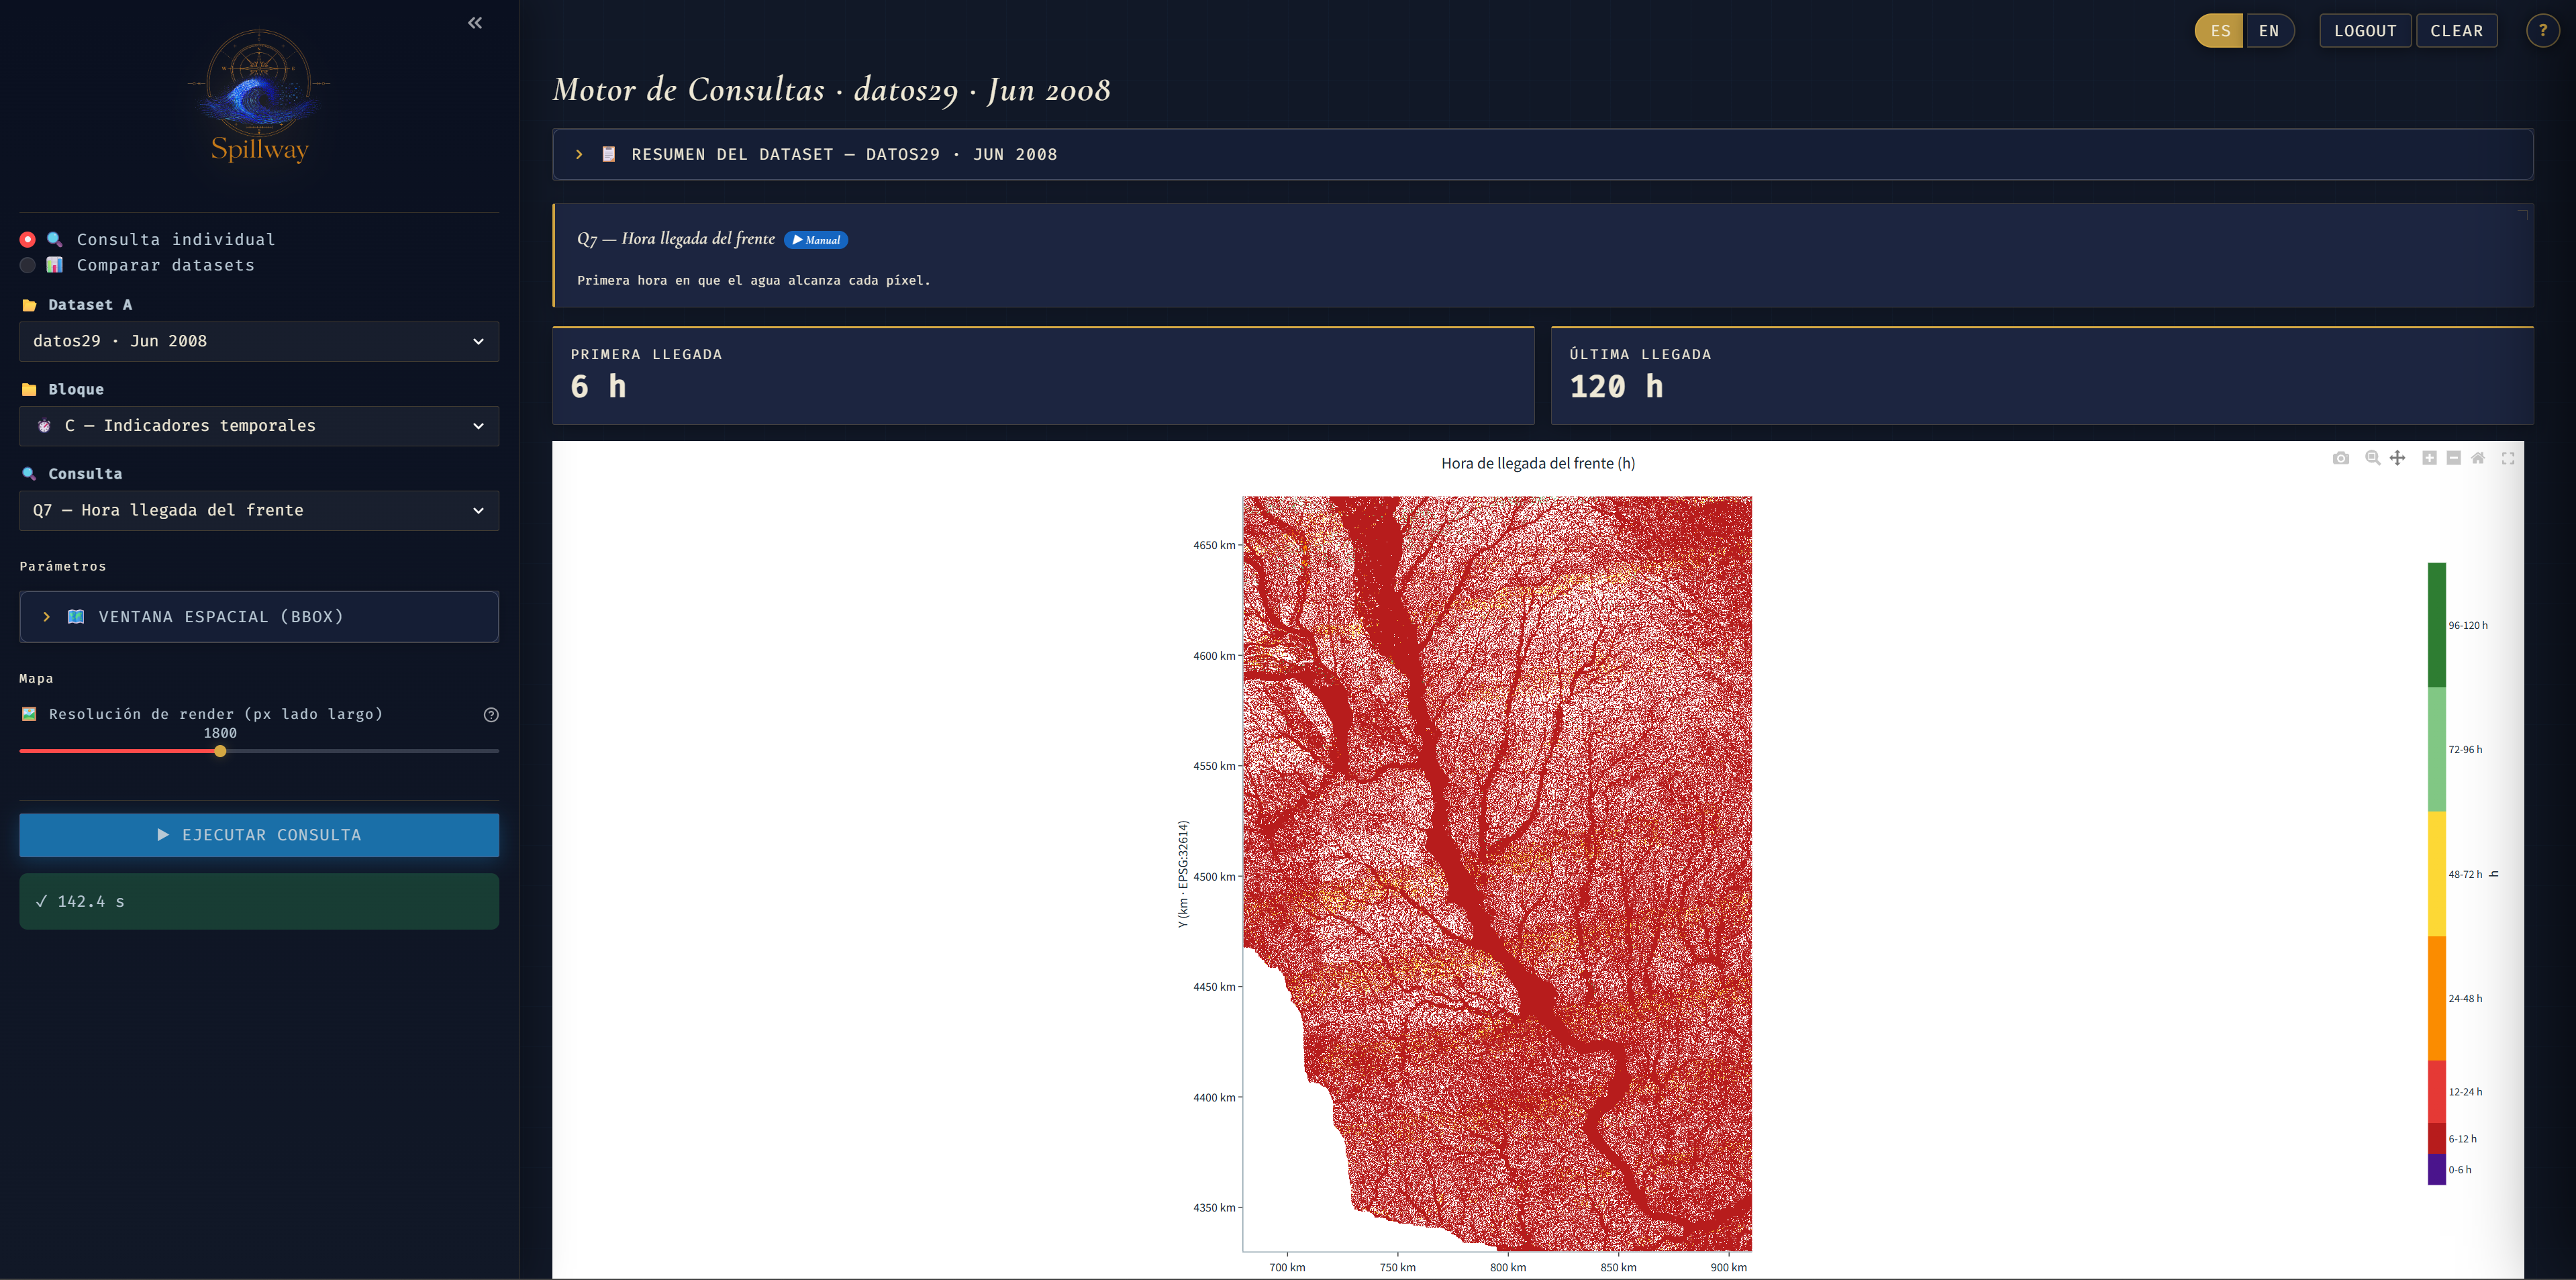
\includegraphics[width=\textwidth]{Imagenes/Captura_Spillway}
\caption{Interfaz de la aplicación Streamlit mostrando la consulta Q7 (hora de llegada del frente de inundación) sobre \texttt{datos29}. La paleta de colores va de púrpura (frente llega antes de 6 h) a verde oscuro (después de 80 h).}
\label{fig:app-streamlit}
\end{figure}

\section{Exportación a GeoTIFF}\label{exportacion-a-geotiff}

La exportación a GeoTIFF responde a la necesidad de interoperabilidad con herramientas SIG externas como QGIS, que no leen directamente el formato TileDB. Encaja en el sistema como paso de salida opcional para análisis fuera del entorno Python.

La exportación reconstruye el ráster denso a partir del array sparse: las celdas húmedas se posicionan según (row, col) y las secas reciben nodata (-9999). El GeoTIFF conserva EPSG:32614 y resolución de 10 m. El script acepta \textit{dataset}, paso temporal, variables y opcionalmente una subregión espacial.

Entrada: dataset, paso temporal y variables. Salida: GeoTIFF georreferenciados ($\sim$257 MB por variable). Limitación: exportar los 20 pasos con las 4 variables produciría $\sim$20 GB, anulando la ventaja de compresión. La herramienta es un complemento puntual para SIG, no un formato de almacenamiento alternativo.

El detalle de cada consulta, organizadas en ocho bloques (A--H), se recoge en la Tabla~\ref{tab:bloques-queries} de la sección~\ref{motor-de-consultas-analiticas} y en el Anexo A. Todas admiten subconjunto espacial (bbox en km) y temporal (paso o rango de pasos).

\section{Motor de consultas analíticas}\label{motor-de-consultas-analiticas}

El motor de consultas analíticas es el núcleo del sistema. Proporciona 24 funciones Python que operan directamente sobre el array TileDB sparse sin exportación previa ni carga completa en memoria. Cada función acepta opcionalmente un parámetro bbox (ventana espacial en EPSG:32614) para restringir el análisis a una subregión.

Las consultas multi-paso (bloque C) emplean acumulación incremental: se mantiene un grid de resolución reducida que se actualiza paso a paso con np.minimum.at, np.maximum.at y np.add.at, manteniendo el consumo de memoria constante ($\sim$10 MB). Las 24 funciones se organizan en ocho bloques (Tabla~\ref{tab:bloques-queries}); el catálogo completo con firma y parámetros se recoge en el Anexo A.


\begin{center}
\begin{tabularx}{\textwidth}{>{\raggedright\arraybackslash}p{3.2cm}>{\raggedright\arraybackslash}p{4.5cm}L}
\toprule
\textbf{Bloque} & \textbf{Funciones} & \textbf{Descripción} \\
\midrule
A. Puntuales & Q1, Q2, Q3 & Calado en punto, serie temporal y velocidad en zona \\
B. Umbrales & Q4, Q5, Q6 & Zonas inundadas, evolución de extensión y umbral configurable \\
C. Temporales & Q7, Q8, Q9, Q11 & Hora de llegada, duración, hora de pico y ventana de emergencia \\
D. Russo et al.\ (2013) & Q10a, Q10b, Q10c, Q11b, Q17 & Inestabilidad adultos/niños/vehículos por umbral simplificado (H, $Q_{mod}$) y semáforo Russo (5 niveles) \\
E. Xia et al.\ (2014/2022) & Q10a-Xia, Q10b-Xia, Q10c-Xia & Inestabilidad adultos/niños por velocidad crítica $U_{c,p}$ y arrastre de vehículos $U_{c,v}$; tres niveles de riesgo \\
F. Estadísticos & Q12, Q13, Q14, Q15 & Área, volumen, estadísticos de zona y semáforo de calado (3 niveles) \\
G. Evacuación & Q16 & Ventana temporal disponible para evacuación por píxel \\
H. Daños normativos & Q18 & Zona de graves daños según RD 9/2008: $H > 1$ m, $V > 1$ m/s ó $H{\cdot}V > 0{,}5$ m$^2$/s \\
\bottomrule
\end{tabularx}
\captionsetup{hypcap=false}\captionof{table}{Organización de las 24 funciones analíticas por bloque.}
\label{tab:bloques-queries}
\end{center}

Los bloques D y E implementan criterios de peligrosidad complementarios. El bloque D emplea umbrales operativos simplificados de Russo et al.\ \cite{russo2013}: una celda es peligrosa para adultos si $H > 0{,}50$ m o $Q_{mod} > 0{,}50$ m²/s, y para niños si $H > 0{,}25$ m o $Q_{mod} > 0{,}15$ m²/s. El bloque E incorpora el criterio experimental de Xia et al.\ \cite{xia2014} para personas y de Xia et al.\ \cite{xia2011vehicles} para vehículos, que calcula para cada celda la velocidad crítica $U_{c,p}(H)$ a partir de la cual el flujo desestabiliza al individuo. Para personas, la fórmula depende de la estatura y masa del individuo ($h_p$, $m_p$) y de seis coeficientes experimentales; cada celda se clasifica en tres niveles: segura ($V < U_{c,p}^{\text{naranja}}$), riesgo moderado ($U_{c,p}^{\text{naranja}} \leq V < U_{c,p}^{\text{roja}}$) y riesgo alto ($V \geq U_{c,p}^{\text{roja}}$). Las dos curvas acotan la incertidumbre experimental del modelo. El criterio de vehículos aplica la misma estructura con la velocidad crítica de arrastre $U_{c,v}(H)$, que varía según el grado de sumersión del vehículo. El bloque H identifica la zona de graves daños según el Real Decreto 9/2008 \cite{rd9_2008}, que establece ese umbral cuando se cumple al menos una de las condiciones $H > 1$ m, $V > 1$ m/s o $H{\cdot}V > 0{,}5$ m²/s.


\section{Comparativa TileDB frente a GeoTIFF}\label{benchmark-vs-geotiff}

Para cuantificar la ventaja práctica del array TileDB sparse frente al acceso directo a los GeoTIFF originales se diseñó un \textit{benchmark} con seis casos de prueba que cubren los patrones de acceso más habituales en análisis hidráulico. Cada caso se ejecuta con ambas tecnologías bajo las mismas condiciones: una primera lectura en frío (sin caché Python previa, aunque el SO puede tener páginas en caché) y tres repeticiones en caliente para medir el tiempo estable. La memoria RAM pico se mide con tracemalloc.

Las pruebas se realizan sobre el array TileDB (ByteShuffle+ZSTD-9, 17\,611 MB) y los GeoTIFF originales de 20 pasos $\times$ 4 variables ($\sim$235 GB). La ventana espacial de referencia es (685 000, 4 335 000) $\rightarrow$ (735 000, 4 385 000) {[}50 $\times$ 50 km, zona húmeda SW del dominio{]} y el paso de referencia es 10\_00 (hora 60 h).

Los resultados se recogen en la Tabla~\ref{tab:bench-datos1}.

\begin{center}
\begin{tabularx}{\textwidth}{>{\raggedright\arraybackslash}p{3.0cm}RRRRRRR}
\toprule
\textbf{Caso}
  & \multicolumn{2}{c}{\textbf{TileDB (s)}}
  & \multicolumn{2}{c}{\textbf{GeoTIFF (s)}}
  & \textbf{Factor}
  & \multicolumn{2}{c}{\textbf{RAM (MB)}} \\
\cmidrule(lr){2-3}\cmidrule(lr){4-5}\cmidrule(lr){7-8}
  & $t_{\text{frío}}$ & $t_{\rm cal}$
  & $t_{\text{frío}}$ & $t_{\rm cal}$
  & & TDB & TIF \\
\midrule
C1. Instante completo   & 3.196 & \textbf{1.831}  & 16.598 & 22.757  & \textbf{12.4}$\times$ TDB & \textbf{2\,328} & 6\,012 \\
C2. Ventana 50$\times$50 km & 0.143 & \textbf{0.080} & 0.832  & 0.251  & \textbf{3.1}$\times$ TDB  & \textbf{158}    & 191 \\
C3. Serie temporal, 1 px & 0.086 & 0.067          & 0.056  & \textbf{0.013} & \textbf{5.3}$\times$ TIF & 90 & \textbf{$<$1} \\
C4. Peligro Russo       & 43.797 & \textbf{41.421} & 270.690 & 293.211 & \textbf{7.1}$\times$ TDB & 3\,980 & \textbf{1\,055} \\
C5. Estadísticos zona   & 0.079 & \textbf{0.047}  & 0.630  & 0.114  & \textbf{2.4}$\times$ TDB  & \textbf{90}     & 191 \\
C6. Exportar ventana    & 0.393 & \textbf{0.296}  & 0.931  & 0.719  & \textbf{2.4}$\times$ TDB  & 230    & \textbf{191} \\
\bottomrule
\end{tabularx}
\captionsetup{hypcap=false}\captionof{table}{Benchmark TileDB vs GeoTIFF sobre datos1 (6 casos, 3 repeticiones en caché caliente). En negrita: mejor valor por fila.}
\label{tab:bench-datos1}
\end{center}

Factor = $t_{\rm cal}$(GeoTIFF) / $t_{\rm cal}$(TileDB) si gana TileDB, o $t_{\rm cal}$(TileDB) / $t_{\rm cal}$(GeoTIFF) si gana GeoTIFF.

\textbf{Análisis de resultados}

TileDB supera a GeoTIFF en cinco de los seis casos de prueba. La ventaja más pronunciada se da en C1 (12,4$\times$), donde TileDB evita leer los píxeles secos que representan el $\sim$92 \% del dominio, mientras que GeoTIFF debe descodificar los rásteres completos (34 200 $\times$ 23 040 px $\times$ 4 vars $\times$ 4 bytes $\approx$ 24 GB por instante).

El caso C4 (cálculo del indicador de peligro de Russo para toda la serie temporal) pone de manifiesto la limitación crítica de GeoTIFF: la lectura de H, QX y QY en modo denso requiere aproximadamente 9,5 GB por paso temporal, lo que provoca que el proceso sea terminado por el sistema operativo (OOM) si se intenta cargar cada ráster completo en memoria. La versión por franjas (chunks de 2 000 filas, $\sim$550 MB pico) evita el OOM pero tarda 293 s frente a los 41 s de TileDB, que solo carga las celdas húmedas ($\sim$8,3 \% del dominio).

El único caso en que GeoTIFF supera a TileDB es C3 (serie temporal de un único píxel, 5,3$\times$ más rápido). Esto se debe a que rasterio resuelve una ventana 1$\times$1 píxel mediante una lectura directa a disco sin descodificación de índice sparse, operación que TileDB no puede optimizar al mismo nivel dado su diseño orientado a consultas multidimensionales sobre conjuntos de celdas.

Respecto al consumo de RAM, TileDB es sistemáticamente más eficiente en todos los casos de lectura masiva (C1: 2 328 MB vs 6 012 MB; C2: 158 MB vs 191 MB). En C4, TileDB usa más RAM (3 980 MB) porque acumula todas las celdas húmedas de los 20 pasos en memoria para el cálculo vectorizado, mientras que la versión por franjas de GeoTIFF procesa de forma secuencial con menor huella.

En cuanto al almacenamiento, la reducción es de 240 490 MB (ficheros GeoTIFF) a 17 611 MB (array TileDB con configuración definitiva), un ahorro del 92,7 \% (ratio 13,7$\times$). Esta compresión se debe principalmente al almacenamiento sparse (solo celdas húmedas) y en menor medida al filtro ByteShuffle+ZSTD-9.

\section{Validación sobre un segundo escenario}\label{validacion-benchmark-datos2}

Para verificar la robustez de los resultados obtenidos con datos1, el benchmark TileDB (ByteShuffle+ZSTD-9) vs GeoTIFF se repitió íntegramente sobre un segundo conjunto de datos (datos2), cargado en el array triton\_results/datos2 mediante el mismo \textit{pipeline} ETL. datos2 contiene 1 303 516 575 celdas húmedas (17 492 MB en TileDB), frente a 1 311 695 098 celdas de datos1 (17 611 MB), lo que indica una simulación con una extensión de inundación ligeramente inferior.

Los resultados se recogen en la Tabla~\ref{tab:bench-datos2}.

\begin{center}
\begin{tabularx}{\textwidth}{p{4.5cm}XXXXX}
\toprule
\textbf{Caso}
  & \textbf{$t_{\rm cal}$ TDB (s)}
  & \textbf{$t_{\rm cal}$ TIF (s)}
  & \textbf{Factor}
  & \multicolumn{2}{c}{\textbf{RAM (MB)}} \\
\cmidrule(lr){5-6}
  & & & & TDB & TIF \\
\midrule
C1. Instante completo   & \textbf{1.783}  & 17.365         & \textbf{9.7}$\times$ TDB  & \textbf{2\,328} & 6\,012 \\
C2. Ventana 50$\times$50 km & \textbf{0.080} & 0.294       & \textbf{3.7}$\times$ TDB  & \textbf{158}    & 191 \\
C3. Serie temporal, 1 px & 0.061          & \textbf{0.011} & \textbf{5.4}$\times$ TIF  & 90              & \textbf{$<$1} \\
C4. Peligro Russo       & \textbf{47.562} & $\sim$471      & \textbf{9.9}$\times$ TDB  & 3\,980          & \textbf{1\,055} \\
C5. Estadísticos zona   & \textbf{0.058}  & 0.214          & \textbf{3.7}$\times$ TDB  & \textbf{90}     & 191 \\
C6. Exportar ventana    & \textbf{0.380}  & 0.799          & \textbf{2.1}$\times$ TDB  & 230             & \textbf{191} \\
\bottomrule
\end{tabularx}
\captionsetup{hypcap=false}\captionof{table}{Benchmark TileDB vs GeoTIFF sobre datos2: validación (3 repeticiones en caché caliente). En negrita: mejor valor por fila.}
\label{tab:bench-datos2}
\end{center}

Factor = $t_{\rm cal}$(GeoTIFF) / $t_{\rm cal}$(TileDB) si gana TileDB, o $t_{\rm cal}$(TileDB) / $t_{\rm cal}$(GeoTIFF) si gana GeoTIFF.

\textbf{Comparativa datos1 vs datos2}


\begin{table}[ht]
\centering
\begin{tabularx}{\textwidth}{p{5cm}XXX}
\toprule
\textbf{Caso} & \textbf{Factor datos1} & \textbf{Factor datos2} & \textbf{Consistencia} \\
\midrule
C1. Instante completo & 12.4$\times$ TDB & 9.7$\times$ TDB & $\checkmark$ TDB gana \\
C2. Ventana 50$\times$50 km & 3.2$\times$ TDB & 3.7$\times$ TDB & $\checkmark$ TDB gana \\
C3. Serie 1 píxel & 5.6$\times$ TIF & 5.4$\times$ TIF & $\checkmark$ TIF gana \\
C4. Peligro Russo & 7.1$\times$ TDB & 9.9$\times$ TDB & $\checkmark$ TDB gana \\
C5. Estadísticos & 2.4$\times$ TDB & 3.7$\times$ TDB & $\checkmark$ TDB gana \\
C6. Exportar GeoTIFF & 2.4$\times$ TDB & 2.1$\times$ TDB & $\checkmark$ TDB gana \\
\bottomrule
\end{tabularx}
\caption{Comparativa del factor de aceleración TileDB vs GeoTIFF entre los datasets datos1 y datos2.}
\label{tab:comparativa-datos1-datos2}
\end{table}


La Tabla~\ref{tab:comparativa-datos1-datos2} compara los factores de aceleración entre ambos \textit{datasets}. Los resultados son consistentes: TileDB supera a GeoTIFF en cinco de los seis casos en las dos simulaciones. La única excepción es C3 (serie temporal de un único píxel), donde GeoTIFF realiza una lectura directa de 1$\times$1 píxel sin necesidad de descomprimir tiles sparse. Esta consistencia valida que las ventajas de TileDB no son específicas de un conjunto de datos concreto, sino inherentes al modelo de almacenamiento sparse frente al acceso denso de los GeoTIFF.

\section{Comparativa multi-escenario}\label{comparativa-multiescenario}

Se ejecutó la comparativa sobre los cuatro \textit{datasets} de referencia (datos1--datos4). La Tabla~\ref{tab:metricas-datasets} recoge las métricas principales. Los resultados confirman que datos1, datos2 y datos4 representan escenarios de inundación de magnitud similar (extensión máxima 7 433--7 718 km\textsuperscript{2}, $\sim$1 300 M celdas húmedas), mientras que datos3 corresponde a un escenario significativamente más seco (extensión máxima 2 838 km\textsuperscript{2}, 498 M celdas). El pico de inundación de datos3 ocurre en la hora 6 frente a las horas 90--96 del resto de datasets. Posteriormente se procesaron los 52 escenarios adicionales (datos5--datos56, junio 1984 a abril 2035) con el mismo \textit{pipeline} ETL, aunque su análisis comparativo queda fuera del alcance de este documento.

\begin{table}[ht]
\centering
\begin{tabularx}{\textwidth}{p{6cm}XXXX}
\toprule
\textbf{Métrica} & \textbf{datos1} & \textbf{datos2} & \textbf{datos3} & \textbf{datos4} \\
\midrule
Pasos temporales & 20 & 20 & 20 & 20 \\
Celdas húmedas totales (M) & 1 311.7 & 1 303.5 & 498.4 & 1 323.5 \\
Extensión máxima (km\textsuperscript{2}) & 7 433 & 7 718 & 2 838 & 7 569 \\
Hora del pico (h) & 90 & 96 & 6 & 96 \\
Extensión en hora 60 (km\textsuperscript{2}) & 6 196 & 6 059 & 2 358 & 6 196 \\
Peligro adultos Russo h60 (km\textsuperscript{2}) & 2 311 & 2 294 & 717 & 2 311 \\
Volumen máximo (Mm\textsuperscript{3}) & 4 462.8 & 4 325.3 & 1 327.9 & 4 462.8 \\
\bottomrule
\end{tabularx}
\caption{Métricas globales por dataset (datos1--datos4).}
\label{tab:metricas-datasets}
\end{table}


La evolución horaria detallada (extensión e indicador de peligro para adultos en cada hora de simulación) se recoge en la Tabla~\ref{tab:evolucion-horaria} del Anexo B.

\section{Aplicación web interactiva}\label{aplicacion-web-interactiva}

La aplicación web constituye la capa de presentación del sistema y el principal punto de acceso para el usuario final. Desarrollada con Streamlit \cite{streamlit}, expone las 20 consultas del motor analítico mediante una interfaz accesible desde el navegador sin instalación adicional de software ni escritura de código.

Al arrancar, la aplicación descubre automáticamente los \textit{datasets} disponibles en el directorio triton\_results/ y permite seleccionar el escenario activo desde la barra lateral. El selector de escenario muestra el alias del \textit{dataset} junto con su fecha de inicio (por ejemplo, datos1 · Jul 1980), extraída automáticamente del nombre del directorio. Un panel colapsable opcional muestra los metadatos del \textit{dataset} seleccionado: número de pasos temporales y duración total, extensión del dominio en km\textsuperscript{2} y resolución espacial.

Las 20 consultas se presentan organizadas en los seis bloques del motor analítico (A--F) como secciones desplegables. Cada consulta muestra una etiqueta de modo (automático/manual) que indica si el resultado se calcula directamente al seleccionar los parámetros o requiere confirmación explícita, distinguiendo así las consultas aptas para uso interactivo de las que implican tiempos de cómputo elevados.

Los resultados se presentan en tres formatos según la naturaleza de la consulta: mapa interactivo Folium para consultas espaciales, gráfico temporal Plotly para series de datos y tabla para estadísticos numéricos. Las consultas de dominio completo (Q12, Q13) emplean @st.cache\_data para evitar recalcular cuando los parámetros no cambian. Las consultas espacialmente acotadas admiten tres modalidades de entrada de coordenadas: selección directa sobre el mapa, introducción manual de coordenadas UTM y carga de un fichero CSV con puntos preprocesados.

La aplicación soporta interfaz bilingüe (español e inglés) seleccionable desde la barra lateral, incluyendo las etiquetas de consulta y los nombres de los bloques analíticos. La aplicación incorpora además un sistema de autenticación por usuario y contraseña que protege el acceso y permite su despliegue en un servidor remoto accesible directamente desde el navegador sin configuración adicional en el cliente.

Entrada: interacción del usuario vía navegador. Salida: mapas interactivos, gráficos temporales, tablas y exportación opcional a GeoTIFF. Limitación: las consultas de dominio completo (Q12, Q13) requieren 30--44 s en la primera ejecución; en despliegues con múltiples usuarios simultáneos el consumo de RAM se multiplica con el número de sesiones activas, lo que aconseja al menos 16 GB de RAM en el servidor.

Las métricas de resumen de cada consulta se han ampliado para ofrecer indicadores operacionalmente relevantes: hora del calado máximo en Q2, calado máximo global en Q9, intensidad máxima relativa al umbral Russo en Q10, ventana máxima practicable en Q11, desviación típica del calado en Q14, área total inundada en Q15, y porcentaje de celdas que alcanzan condición crítica al primer instante de inundación en Q16. Se corrigió además la máscara de Q11, que ahora restringe correctamente las celdas al rango $H \geq 0{,}01$ m y $H < 0{,}60$ m, consistente con la definición del criterio de vehículos de emergencia.

Las consultas de múltiples pasos temporales (Q7, Q8, Q9, Q11 y Q16) emplean un grid acumulador de tipo entero sin signo de 8 bits, de dimensiones fijas nr x nc, que se actualiza incrementalmente mediante operaciones np.minimum.at y np.add.at. Este enfoque mantiene el consumo de memoria en torno a 750 MB independientemente del volumen de celdas húmedas, frente a los más de 14 GB que requería la concatenación de listas al procesar 61 millones de celdas por paso sobre el dominio completo. La reducción del tiempo de ejecución de Q7 sobre el dominio completo fue del 55\%, de 200 s a 89 s.

